\documentclass{beamer}
\usepackage[UTF8]{ctex}
\usetheme{Warsaw}  % 样式

\author{Zhan San\\张三}
\date{\today}
\institute{XXX University}

\title{Beamer 制作幻灯片}

\begin{document}

\maketitle

\section{第一节}

\begin{frame}
    \frametitle{页标题}

    \begin{itemize}
        \item 第一条 \pause
        \item \alert{第二条} \pause
        \item 第三条
        \item 第四条
    \end{itemize}

\end{frame}

\begin{frame}
    \frametitle{本页标题}

    第二页内容
    \begin{theorem}[勾股定理]
        $$c^2 = b^2 + c^2$$
    \end{theorem}

\end{frame}

\begin{frame}
    \frametitle{第三页}
    \begin{figure}
        \centering
        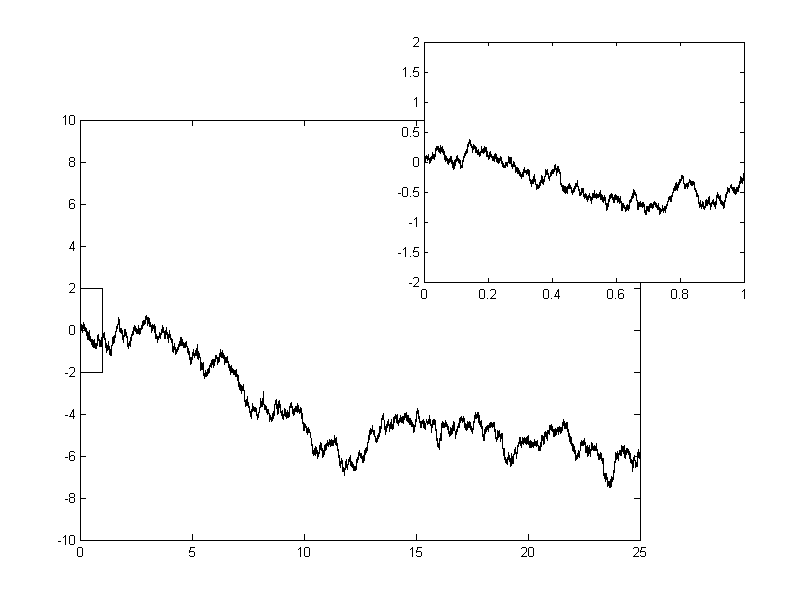
\includegraphics[width=0.6\textwidth]{Wiener_process_zoom.png}

        \caption{Wiener process.}
        \label{}
    \end{figure}
    
\end{frame}

\begin{frame}
    \frametitle{}
    \centering
    \zihao{0}  % 字号设置 详见ctex文档第8节
    谢谢!
\end{frame}

\end{document}